\section{Experimental Evaluation}

\begin{frame}
	\frametitle{Experimental Evaluation}
	\framesubtitle{Data sets}
	
	\Large
	
	\vspace{0.5cm}
	
	We carried out experiments on the Alzheimer's Disease Neuroimaging Initiative$^1$  (ADNI) data set
	and on the publicly available Open Access Series of Imaging Studies$^2$ (OASIS) data set
	
	\begin{center}
		\begin{tikzpicture}
			\node at (-4,0) [draw=red,ultra thick,inner sep=0pt]
			{
				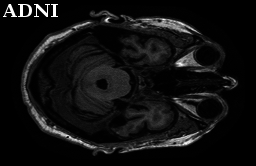
\includegraphics[height=3cm]{Figures/ADNI}
			};
			\node at (0,0) [draw=red,ultra thick,inner sep=0pt]
			{
				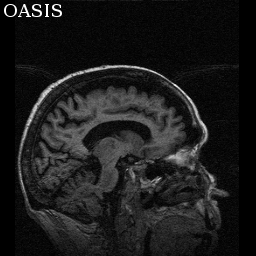
\includegraphics[height=3cm]{Figures/OASIS}
			};
		\end{tikzpicture}
	\end{center}
	
	\vspace{-0.05cm}
	
	\tiny
	
	$^1$ \url{http://adni.loni.usc.edu}
	
	$^2$ \url{http://www.oasis-brains.org}
\end{frame}

\begin{frame}
	\frametitle{Experimental Evaluation}
	\framesubtitle{Results on ADNI}
	
	\small
	
	\vspace{-0.1cm}
	
	\begin{table}
		\centering
		\renewcommand{\arraystretch}{1.3}
		\setlength{\tabcolsep}{0.05cm}
		\begin{tabular}{cc|ccccc}
			\multicolumn{2}{c|}{\textbf{Classes}} & \multicolumn{5}{c}{\textbf{\begin{tabular}[c]{@{}c@{}}
			ADNI \end{tabular}}} \\ \hline
			\textbf{\#} & \textbf{Typology} & \multicolumn{1}{c}{\begin{tabular}[c]{@{}c@{}}Guerrero \\
			\emph{et al.} \cite{Guerrero14} \end{tabular}} &
			\multicolumn{1}{c}{\begin{tabular}[c]{@{}c@{}}Beheshti \\ \emph{et al.} \cite{Beheshti16}
			\end{tabular}} & \multicolumn{1}{c}{\begin{tabular}[c]{@{}c@{}}Zhou \\ \emph{et al.}
			\cite{Zhou14} \end{tabular}} &
			\multicolumn{1}{c}{\begin{tabular}[c]{@{}c@{}}Plocharski \\ \emph{et al.}
			\cite{Plocharski16} \end{tabular}} & \multicolumn{1}{c}{Ours} \\
			\hline
			\multirow{3}{*}{2} & AD,CN & (84,85,84) & (96,98,94) & (92,96,84) & (88,87,90) &
			\textbf{(100,100,99)} \\
			& LMCI,CN & (82,83,81) & - & (75,83,61) & - & \textbf{(100,100,100)} \\
			& LMCI,MCI & (69,60,77) & - & - & - & \textbf{(99,99,99)} \\
			\hline
			3 & AD,MCI,CN & - & - & - & - & \textbf{(98,98,98)} \\
			\hline
			4 & AD,LMCI,MCI,CN & - & - & - & - & \textbf{(99,99,99)}
		\end{tabular}
	\end{table}
	
	\tiny
	
	\cite{Guerrero14} R. Guerrero \emph{et al.}, ``Manifold population modeling as a neuro-imaging
	biomarker: application to ADNI and ADNI-GO'',\\ \hspace{0.25cm} Journal on NeuroImage, 2014
	
	\cite{Beheshti16} I. Beheshti \emph{et al.}, ``Feature-ranking-based Alzheimer's disease
	classification from structural MRI'', Journal on Magnetic\\ \hspace{0.25cm} Resonance Imaging, 2016
	
	\cite{Zhou14} Q. Zhou \emph{et al.}, ``An optimal decisional space for the classification of 
	Alzheimer's disease and mild cognitive impairment'',\\ \hspace{0.25cm} Journal on Biomedical
	Engineering, 2014
	
	\cite{Plocharski16} M. Plocharski \emph{et al.}, ``Extraction of sulcal medial surface and
	classification of Alzheimer's disease using sulcal features'',\\ \hspace{0.25cm} Journal on
	Computer Methods and Programs in Biomedicine, 2016
\end{frame}

\begin{frame}
	\frametitle{Experimental Evaluation}
	\framesubtitle{Results on OASIS}
	
	\small
	
	\vspace{0.6cm}
	
	\begin{table}
		\centering
		\renewcommand{\arraystretch}{1.3}
		\setlength{\tabcolsep}{0.05cm}
		\begin{tabular}{cc|cccc}
			\multicolumn{2}{c|}{\textbf{Classes}} & \multicolumn{4}{c}{\textbf{\begin{tabular}[c]{@{}c@{}}
			OASIS \end{tabular}}} \\ \hline
			\textbf{\#} & \textbf{Typology} & \begin{tabular}[c]{@{}c@{}}Daliri\\ \cite{Daliri12}
			\end{tabular} & \multicolumn{1}{c}{\begin{tabular}[c]{@{}c@{}}Ramaniharan\\ \emph{et al.}
			\cite{Ramaniharan16} \end{tabular}} & \multicolumn{1}{c}{\begin{tabular}[c]{@{}c@{}}Anandh\\
			\emph{et al.} \cite{Anandh16} \end{tabular}} & \multicolumn{1}{c}{Ours} \\
			\hline
			\multirow{3}{*}{2} & AD,CN & - & (93,93,93) & \textbf{(98,98,97)} & (97,97,93) \\
			& LMCI,CN  & - & - & (95,96,94) & \textbf{(96,96,97)} \\
			& LMCI,MCI & - & - & - & \textbf{(83,83,90)} \\
			\hline
			3 & AD,MCI,CN & (78,-,-) & - & - & \textbf{(85,85,86)} \\
			\hline
			4 & AD,LMCI,MCI,CN & (75,-,-) & - & - & \textbf{(77,77,79)}
		\end{tabular}
	\end{table}
	
	\vspace{0.2cm}
	
	\tiny
	
	\cite{Daliri12} M. R. Daliri, ``Automated diagnosis of Alzheimer disease using the scale-invariant
	feature transforms in magnetic resonance\\ \hspace{0.25cm} images'', Journal on Medical Systems,
	2012
	
	\cite{Ramaniharan16} A. K. Ramaniharan \emph{et al.}, ``Laplace Beltrami eigen value based
	classification of normal and Alzheimer MR images using\\ \hspace{0.25cm} parametric and non
	parametric classifiers'', Journal on Expert Systems with Applications, 2016
	
	\cite{Anandh16} K. R. Anandh \emph{et al.}, ``A method to differentiate mild cognitive impairment
	and Alzheimer in MR images using eigen value\\ \hspace{0.25cm} descriptors'', Journal on Medical
	Systems, 2016
\end{frame}

\begin{frame}
	\frametitle{Experimental Evaluation}
	\framesubtitle{Interesting discovery}
	
	\Large
	
	\vspace{0.4cm}
	
	We investigate the \textbf{correlation} between \textbf{classification success} and \textbf{age of
	the patients} and we found out that, there \textbf{is no such a correlation} but, instead, a
	correlation between classification success and state of the disease.
	
	\vspace{0.3cm}
	
	Features extracted from the MRI brain scan relates to the state of the patient's disease and they
	are somehow the same in a young patient and in a elderly one
\end{frame}
